\clearpage
\begingroup
\setcounter{figure}{0}
\renewcommand{\figurename}{Extended Data Fig.}
\renewcommand{\theHfigure}{extended.\arabic{figure}}

\begin{figure}[p]
\section*{Extended Data}
\centering
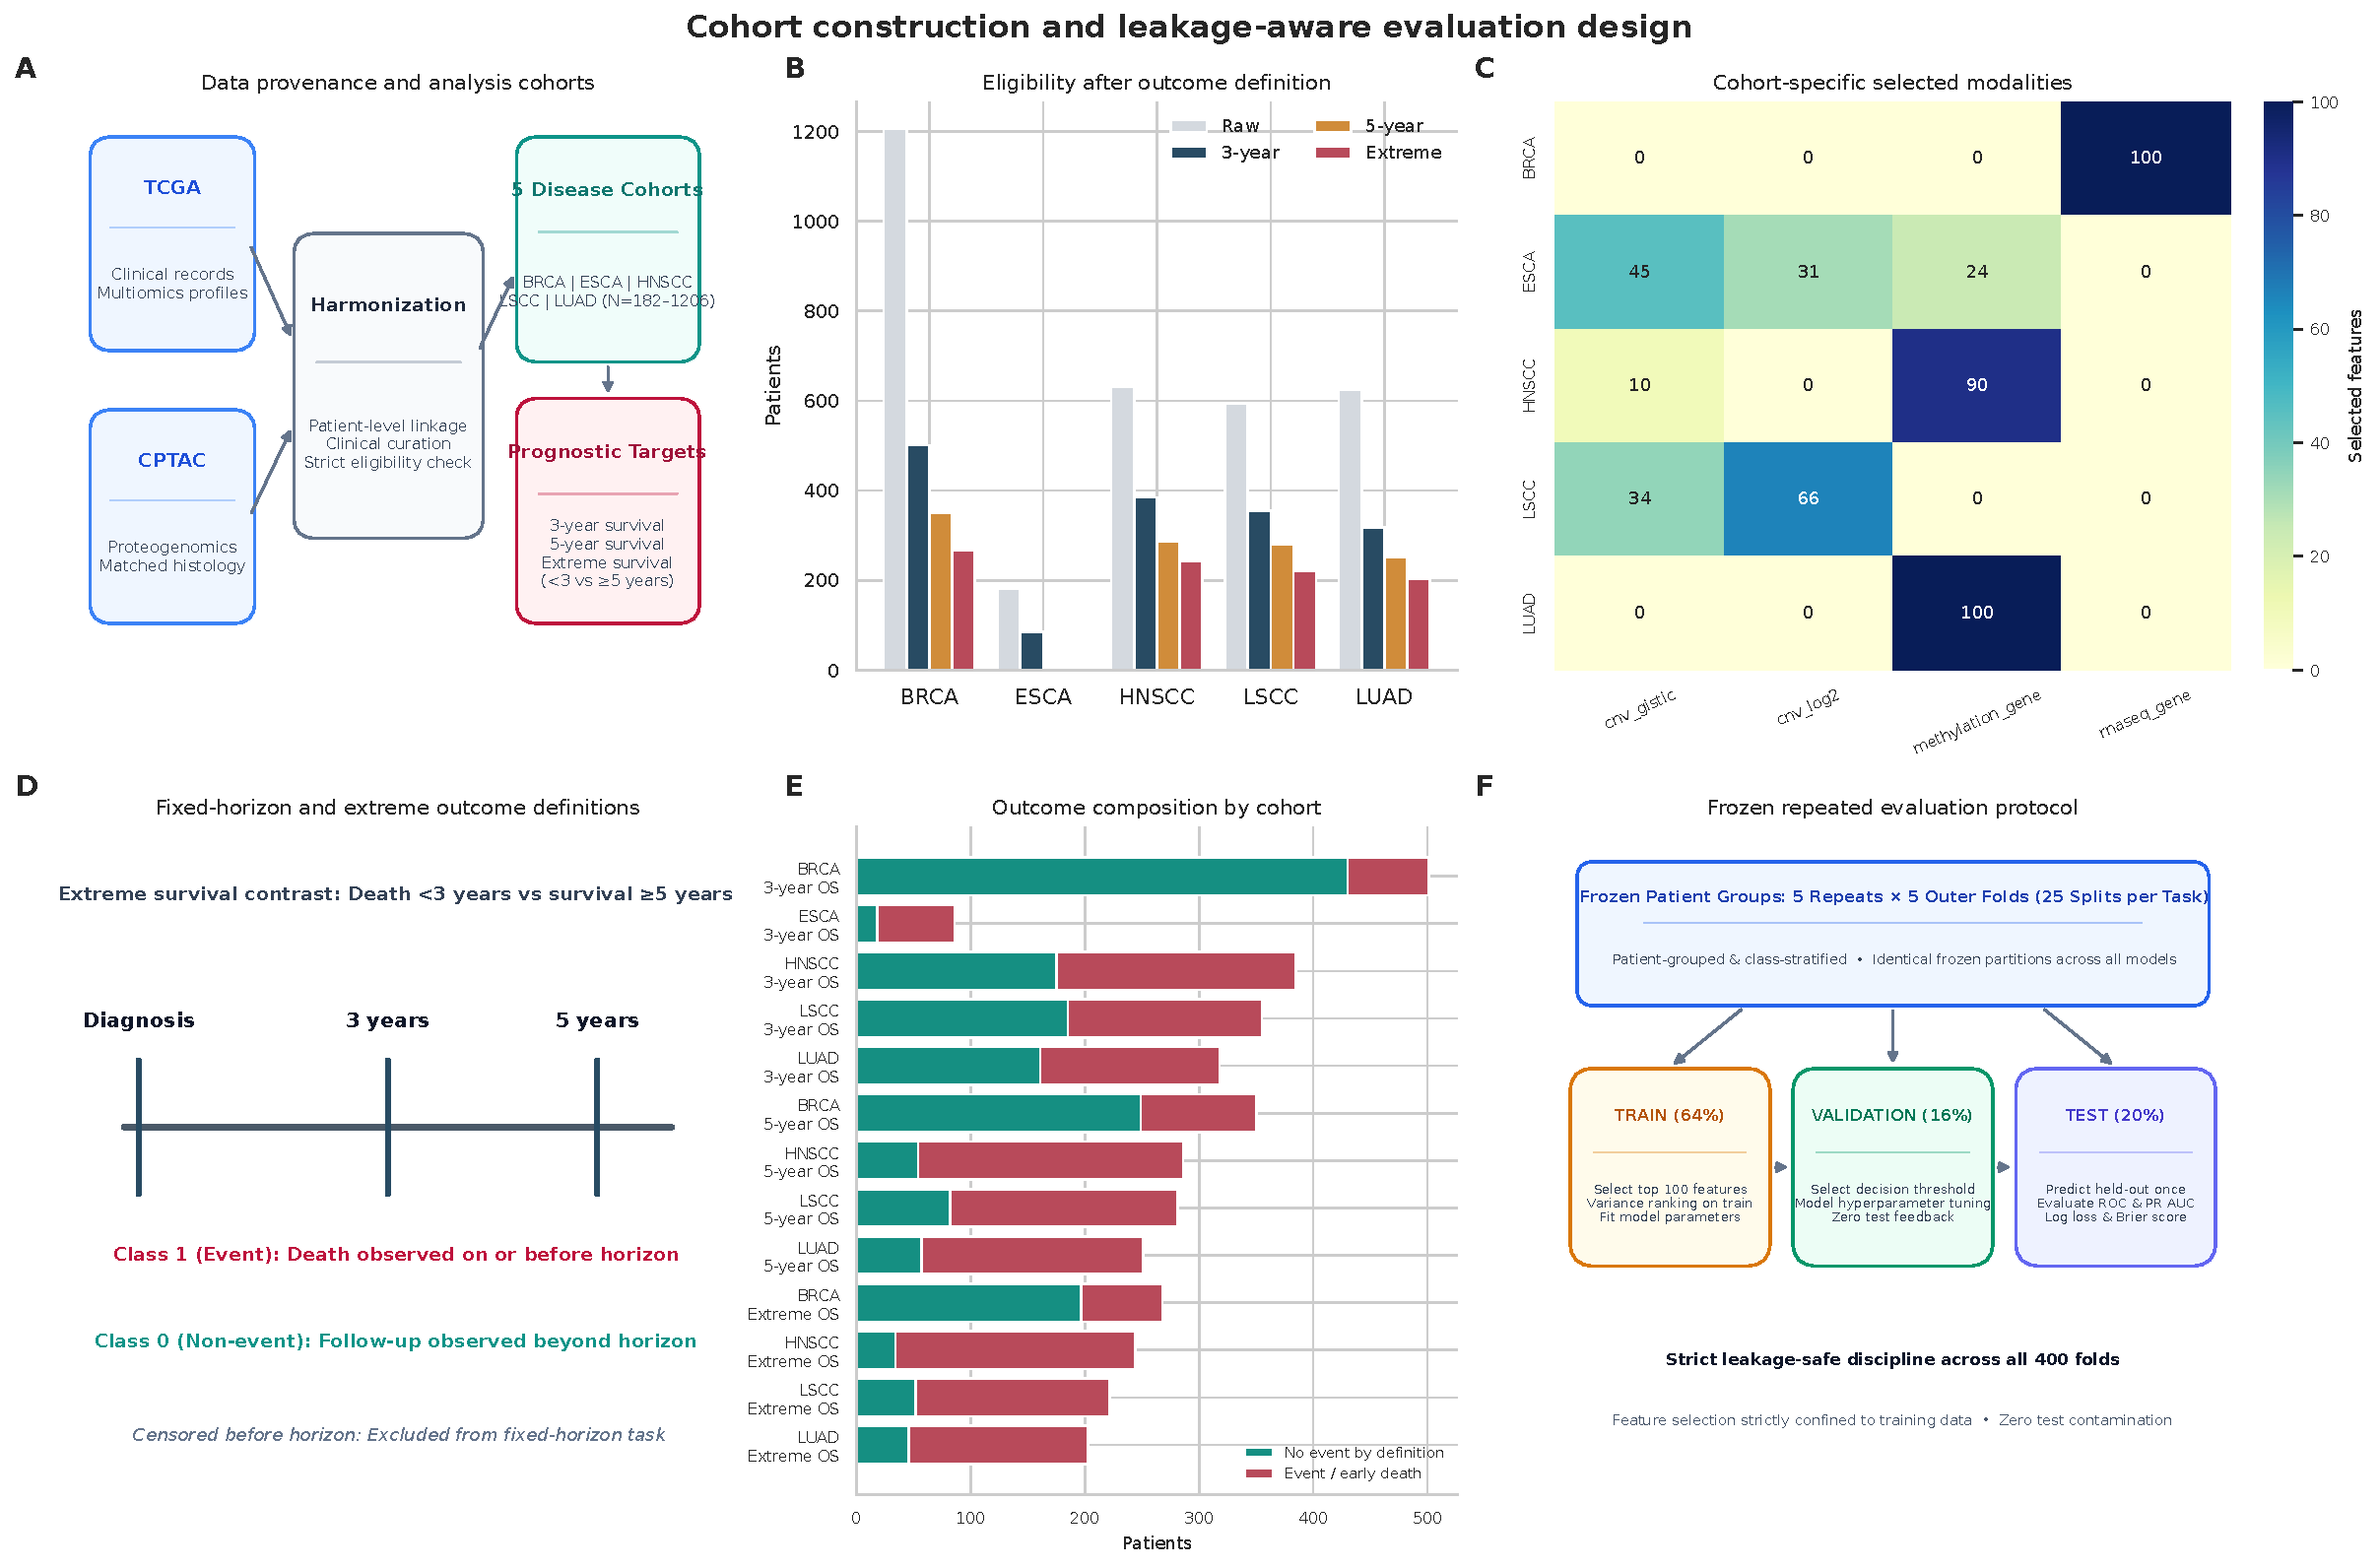
\includegraphics[width=\linewidth,height=0.64\textheight,keepaspectratio]{figures/manuscript/figure_01_cohort_and_design.pdf}
\caption{\textbf{Cohort detail.} Provenance, eligibility, molecular modality composition, endpoint definitions, class counts and the evaluation protocol for the five cohorts.}
\label{fig:ed_cohort}
\end{figure}

\begin{figure}[p]
\centering
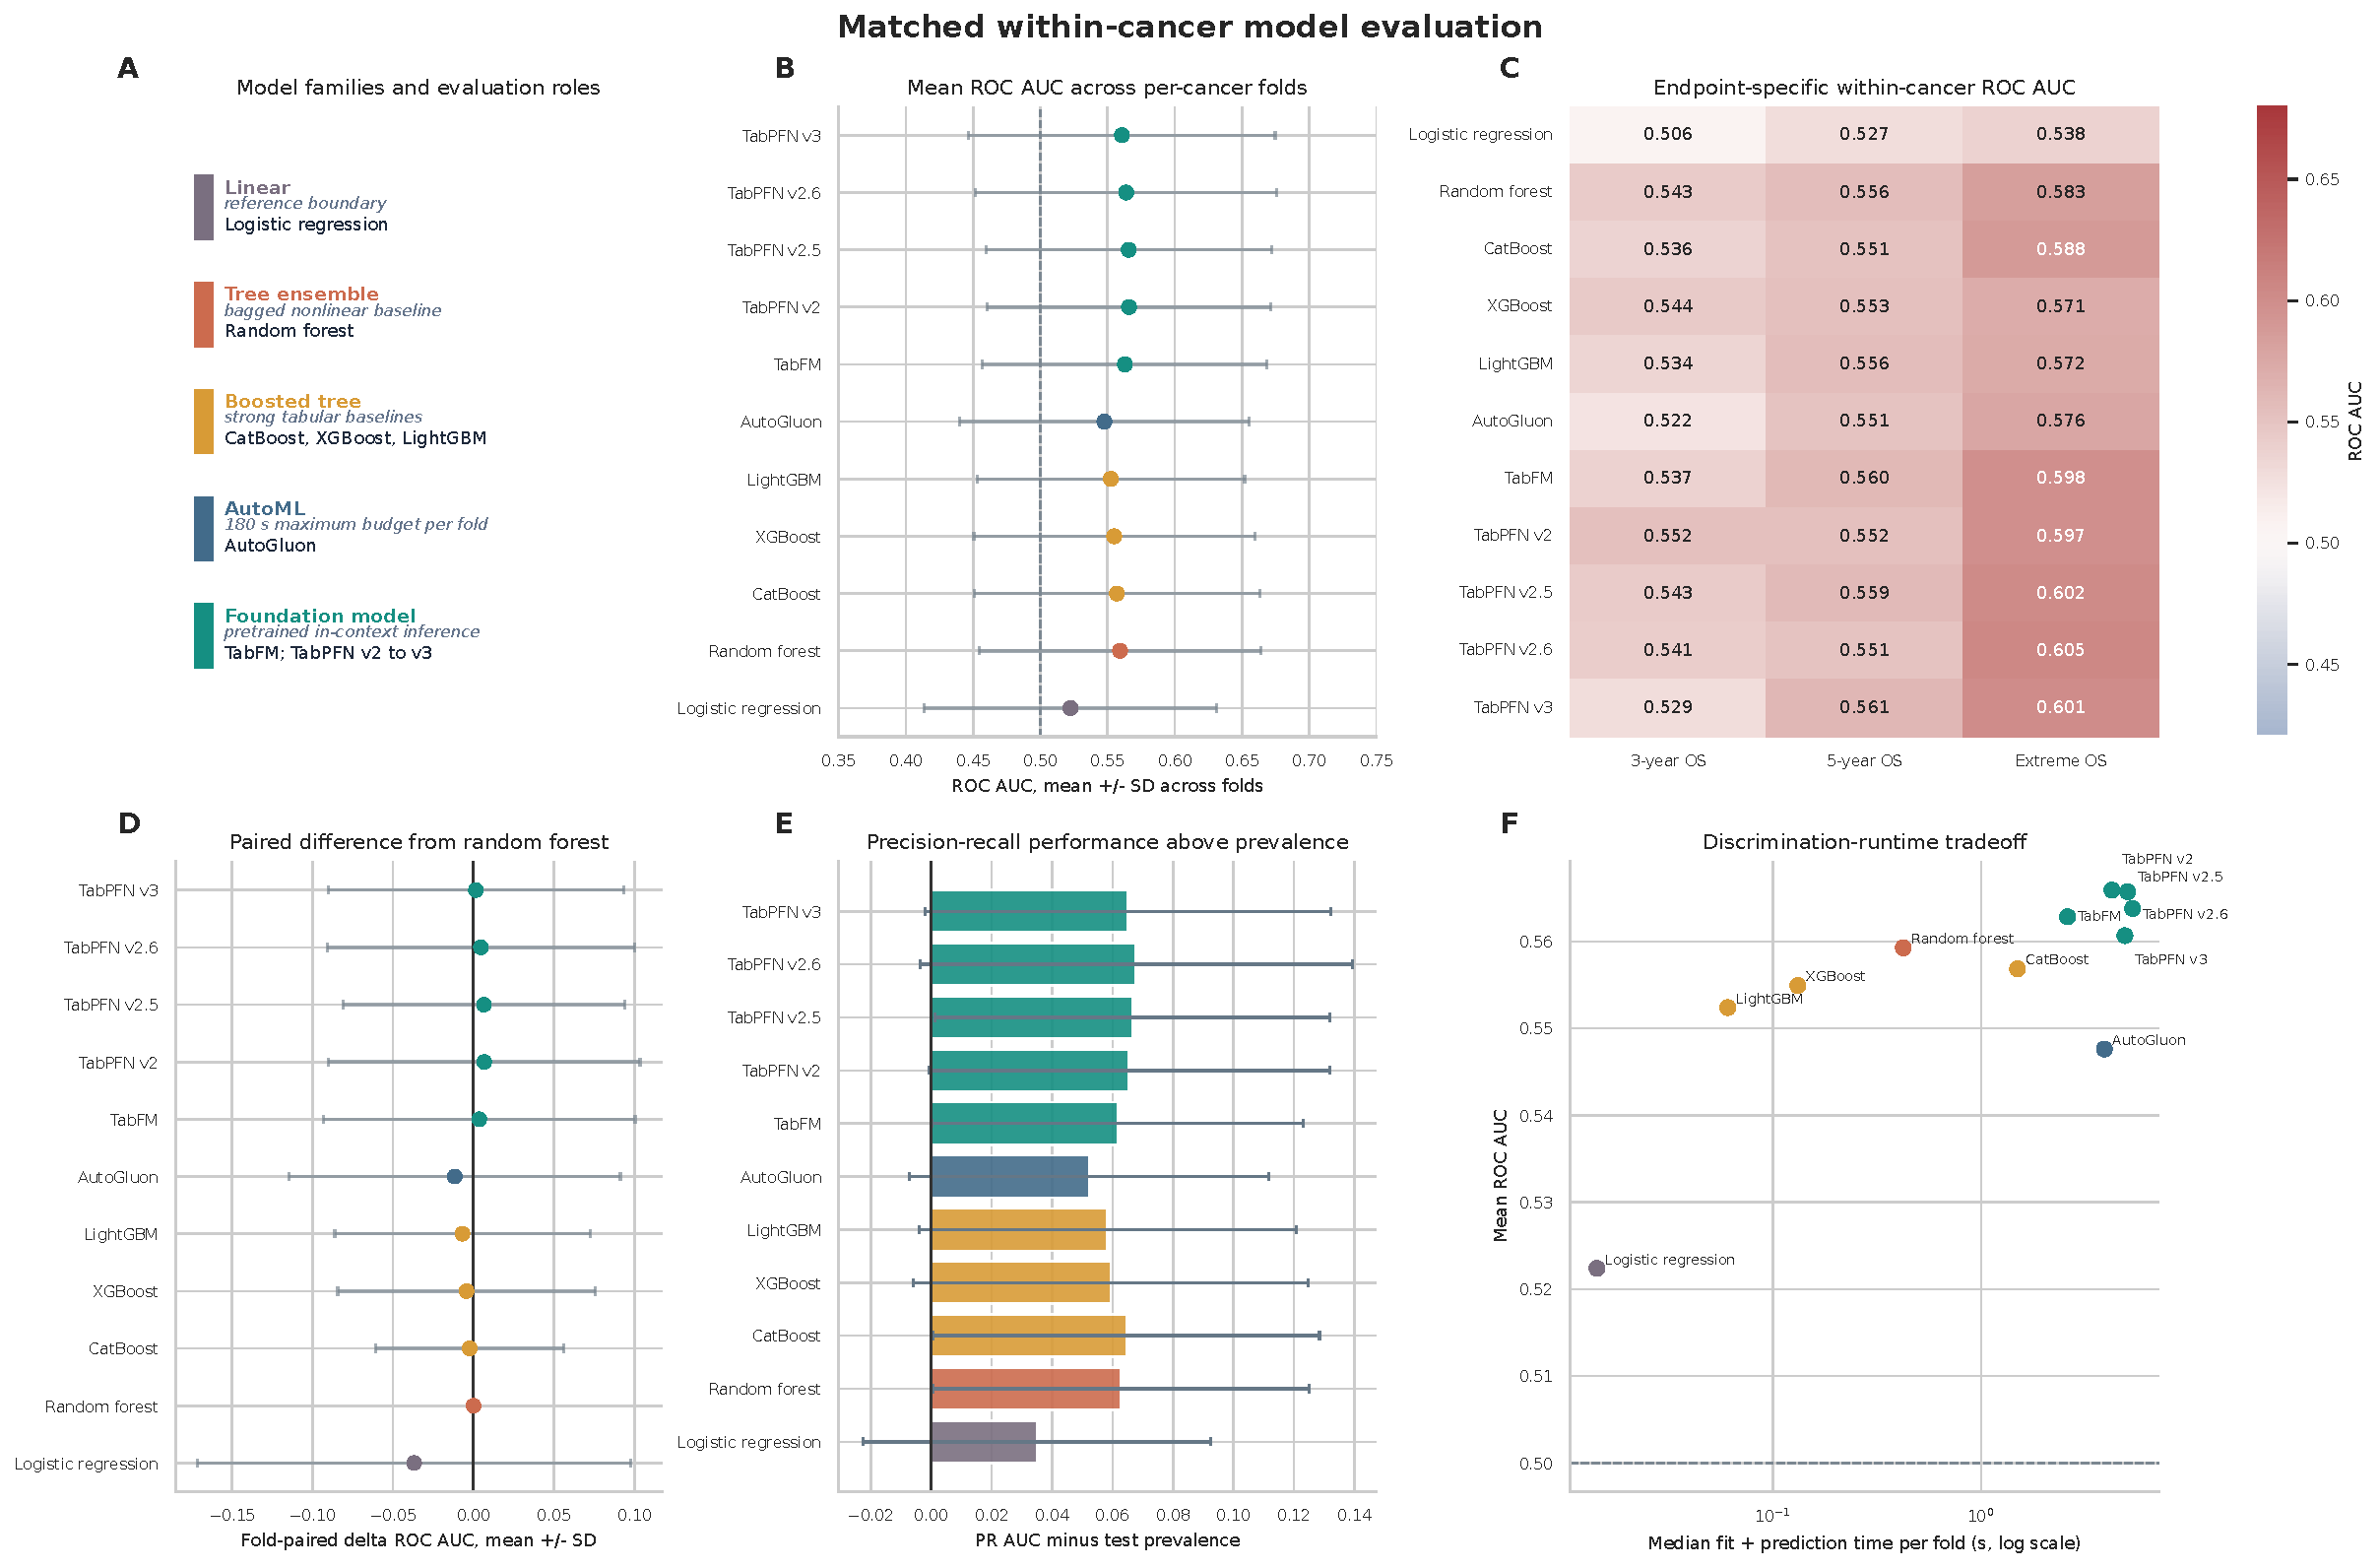
\includegraphics[width=\linewidth,height=0.64\textheight,keepaspectratio]{figures/manuscript/figure_02_within_cancer_performance.pdf}
\caption{\textbf{Within-cancer performance detail.} Model families, mean ROC AUC with variation across test sets, AUC by model and endpoint, fold-matched differences from random forest, precision-recall AUC above prevalence, and runtime.}
\label{fig:ed_within}
\end{figure}

\begin{figure}[p]
\centering
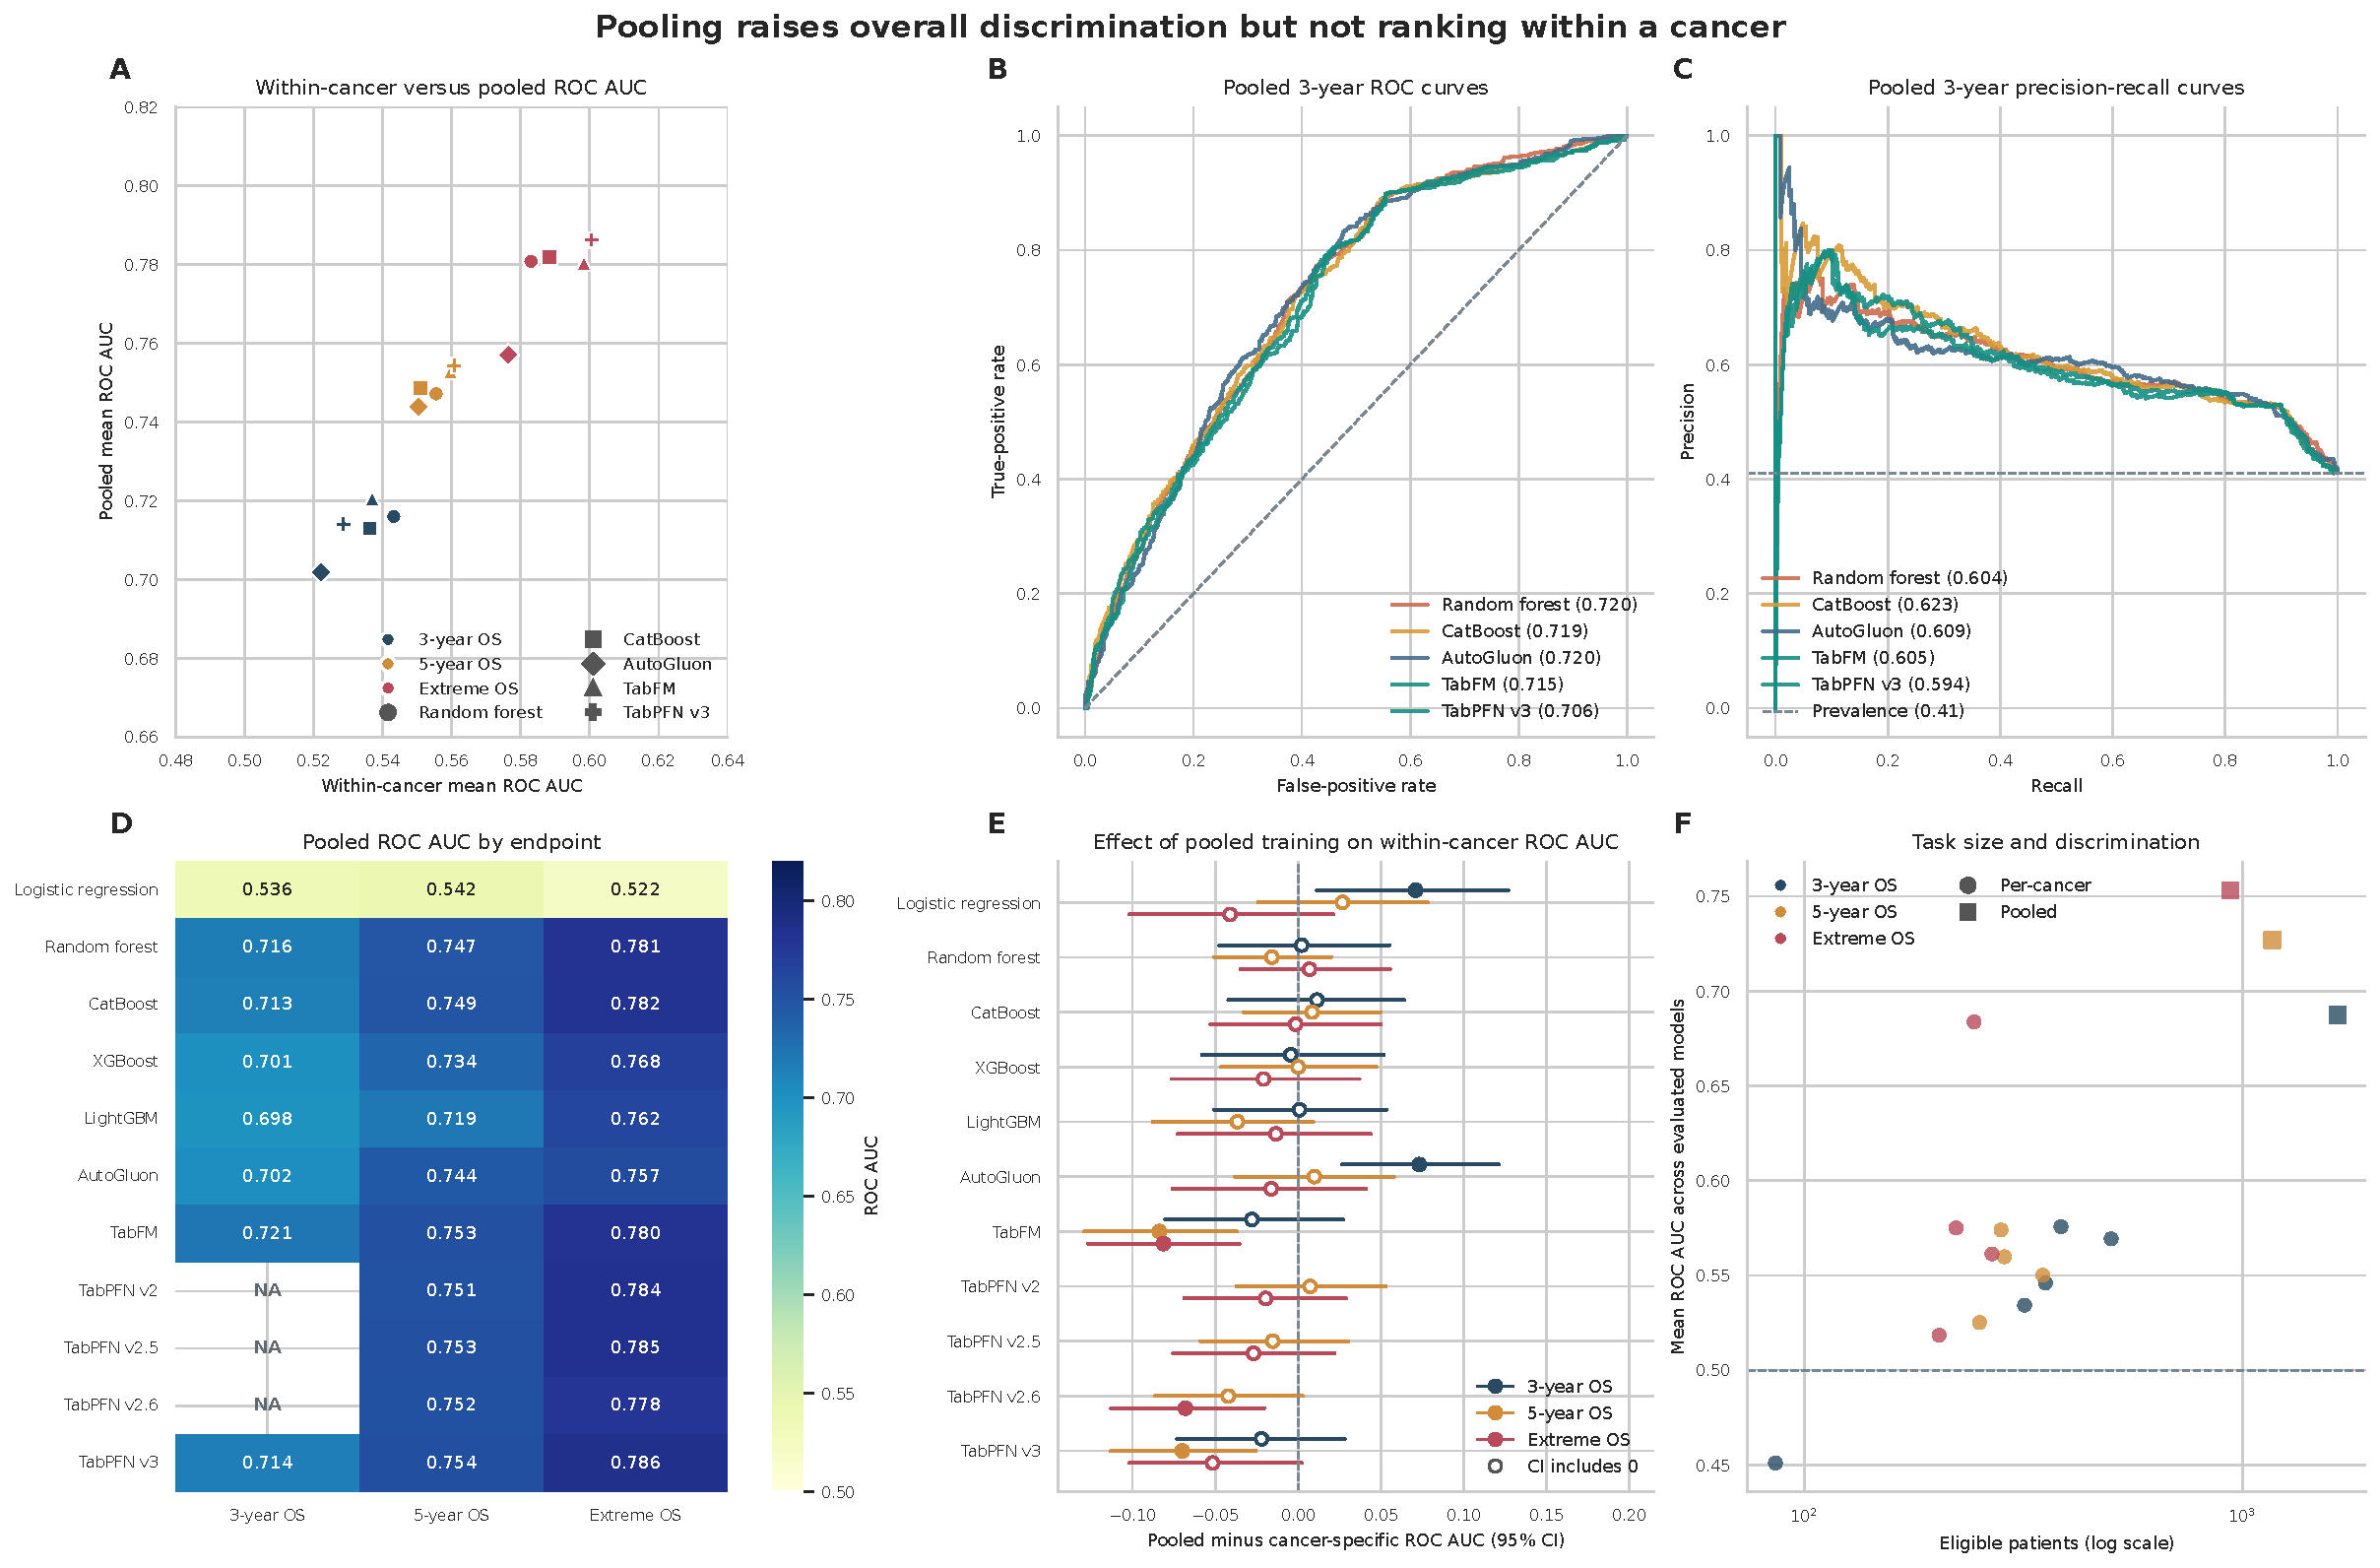
\includegraphics[width=\linewidth,height=0.64\textheight,keepaspectratio]{figures/manuscript/figure_03_pooling_effect.pdf}
\caption{\textbf{Pooled-task curves.} Within-cancer versus pooled AUC, pooled 3-year ROC and precision-recall curves, pooled AUC heatmap, the paired within-cancer effect (first version) and task size against discrimination.}
\label{fig:ed_pool}
\end{figure}

\begin{figure}[p]
\centering
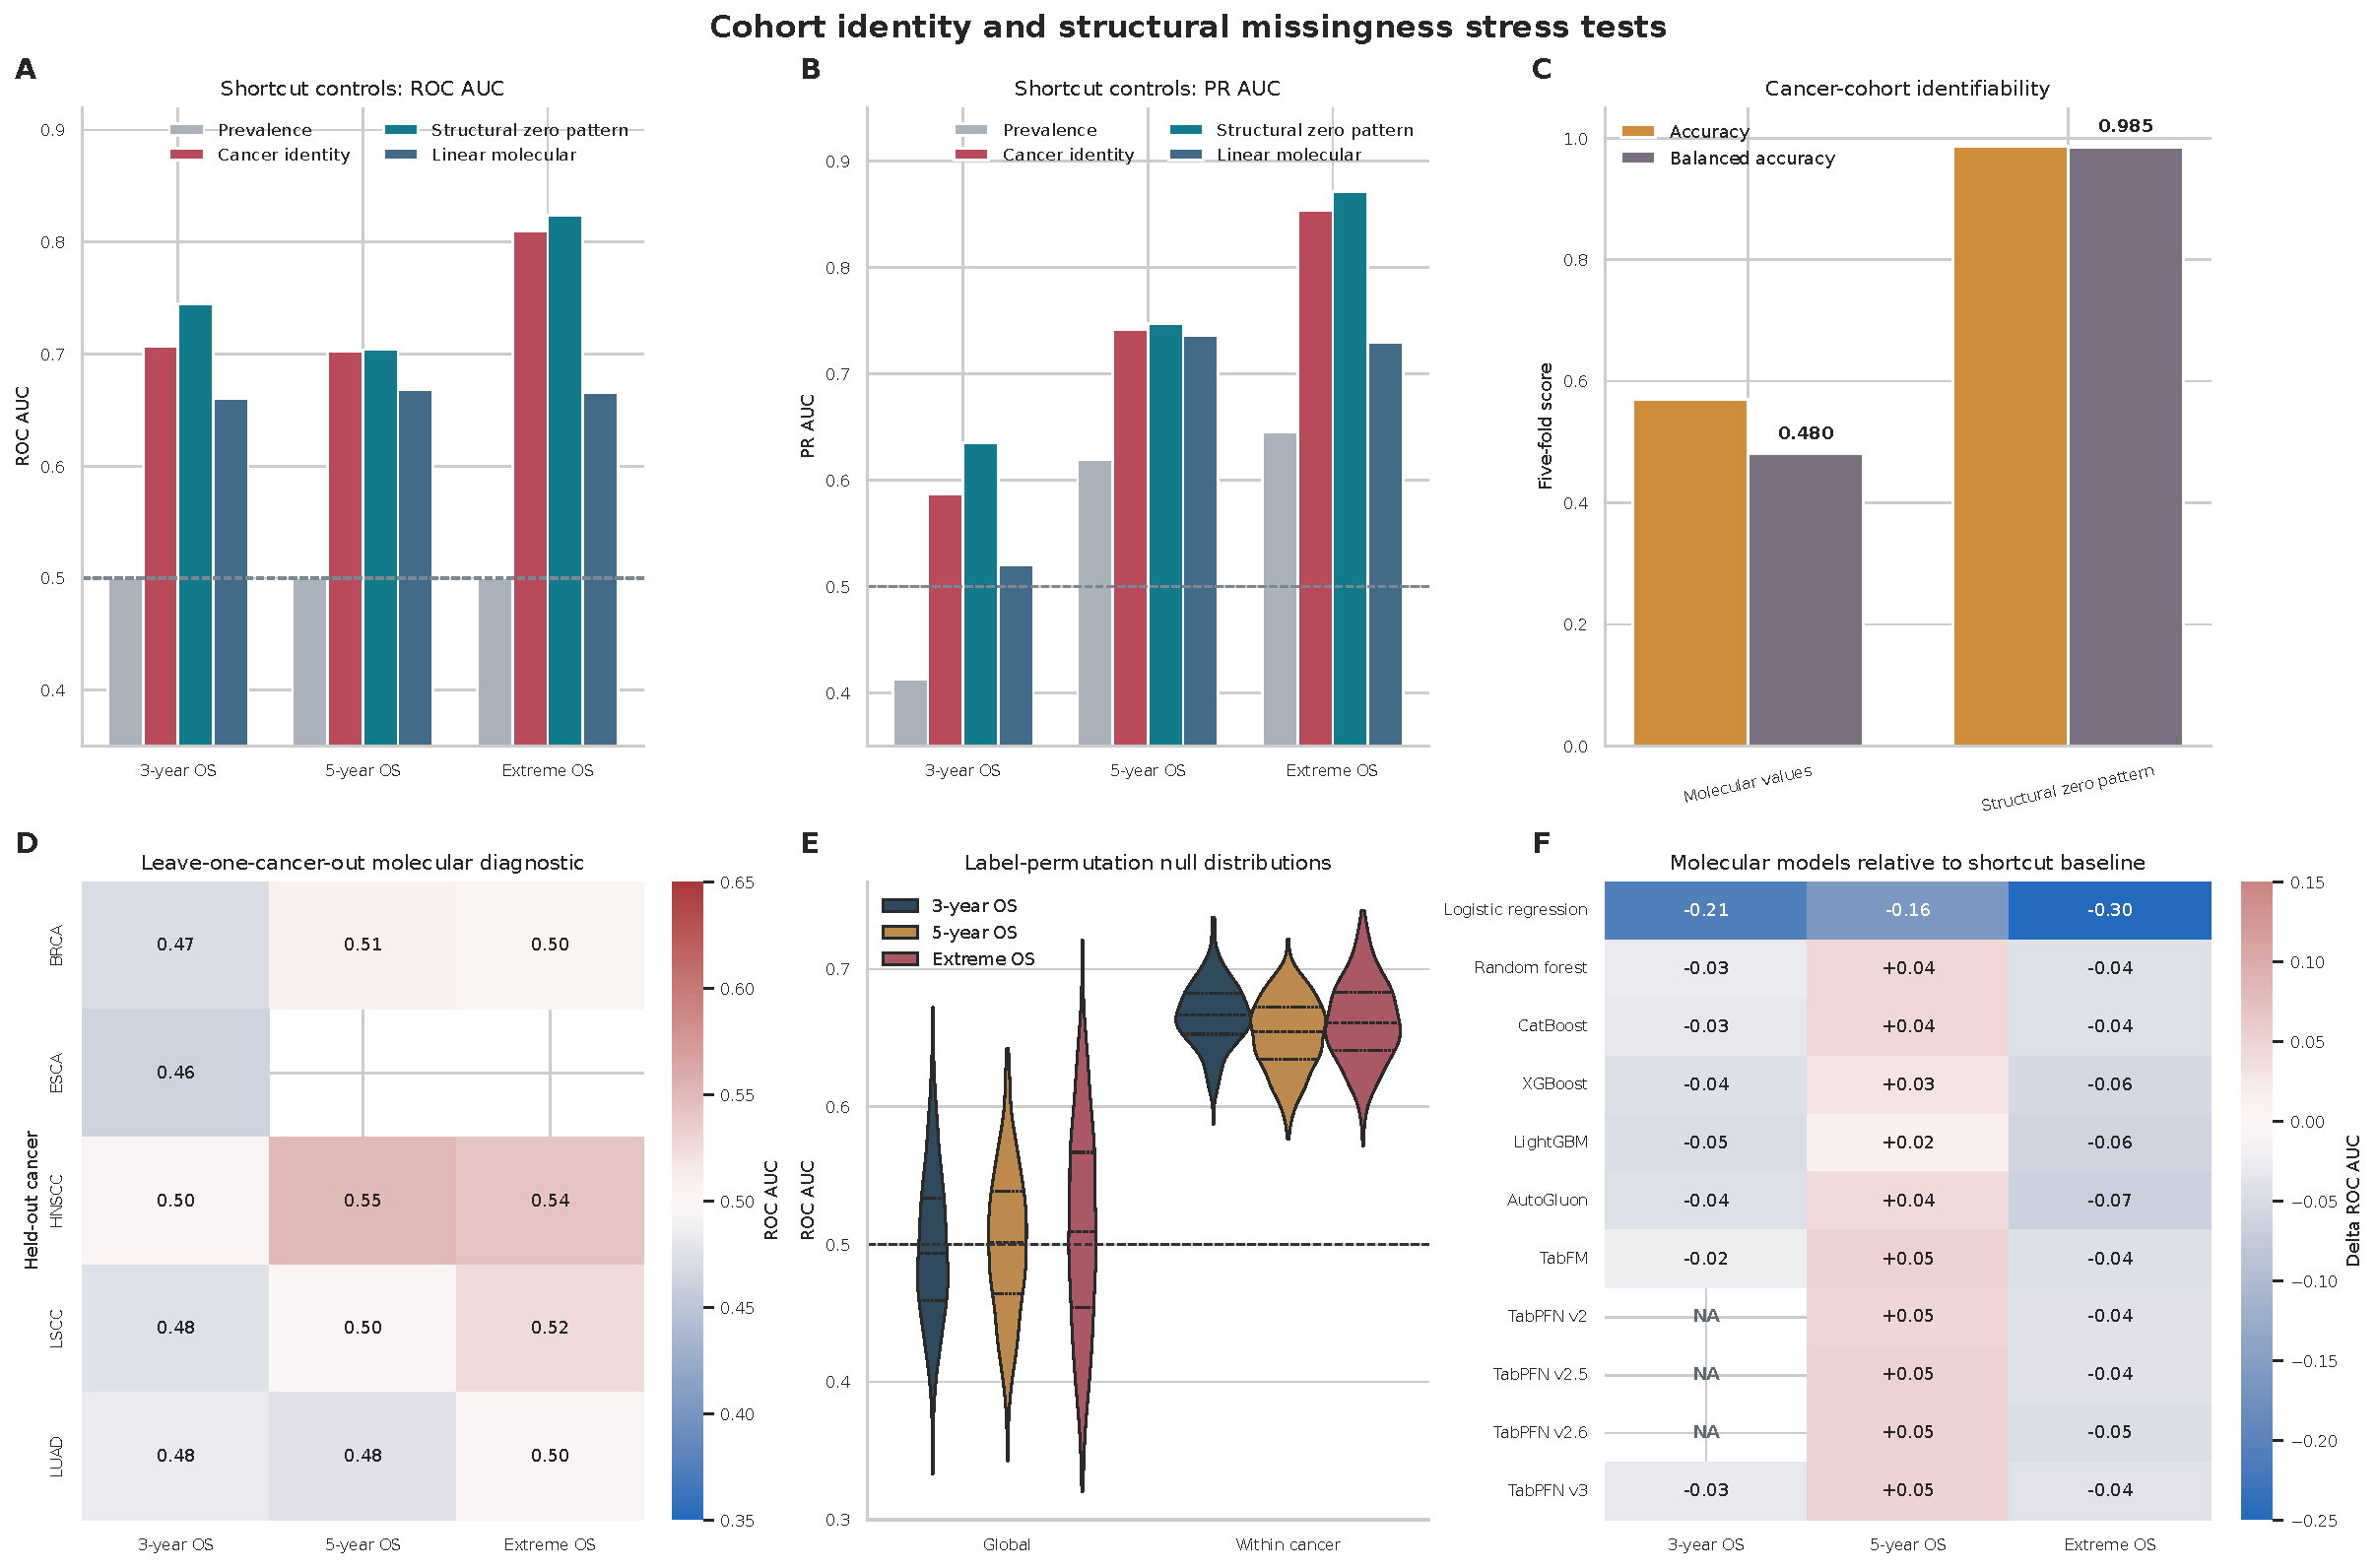
\includegraphics[width=\linewidth,height=0.64\textheight,keepaspectratio]{figures/manuscript/figure_04_shortcut_stress_tests.pdf}
\caption{\textbf{Shortcut-control detail.} Cancer-type and zero-pattern controls, cohort identifiability, cancer-held-out diagnostics, permutation distributions and the difference between each pooled model and the strongest control.}
\label{fig:ed_shortcut}
\end{figure}

\begin{figure}[p]
\centering
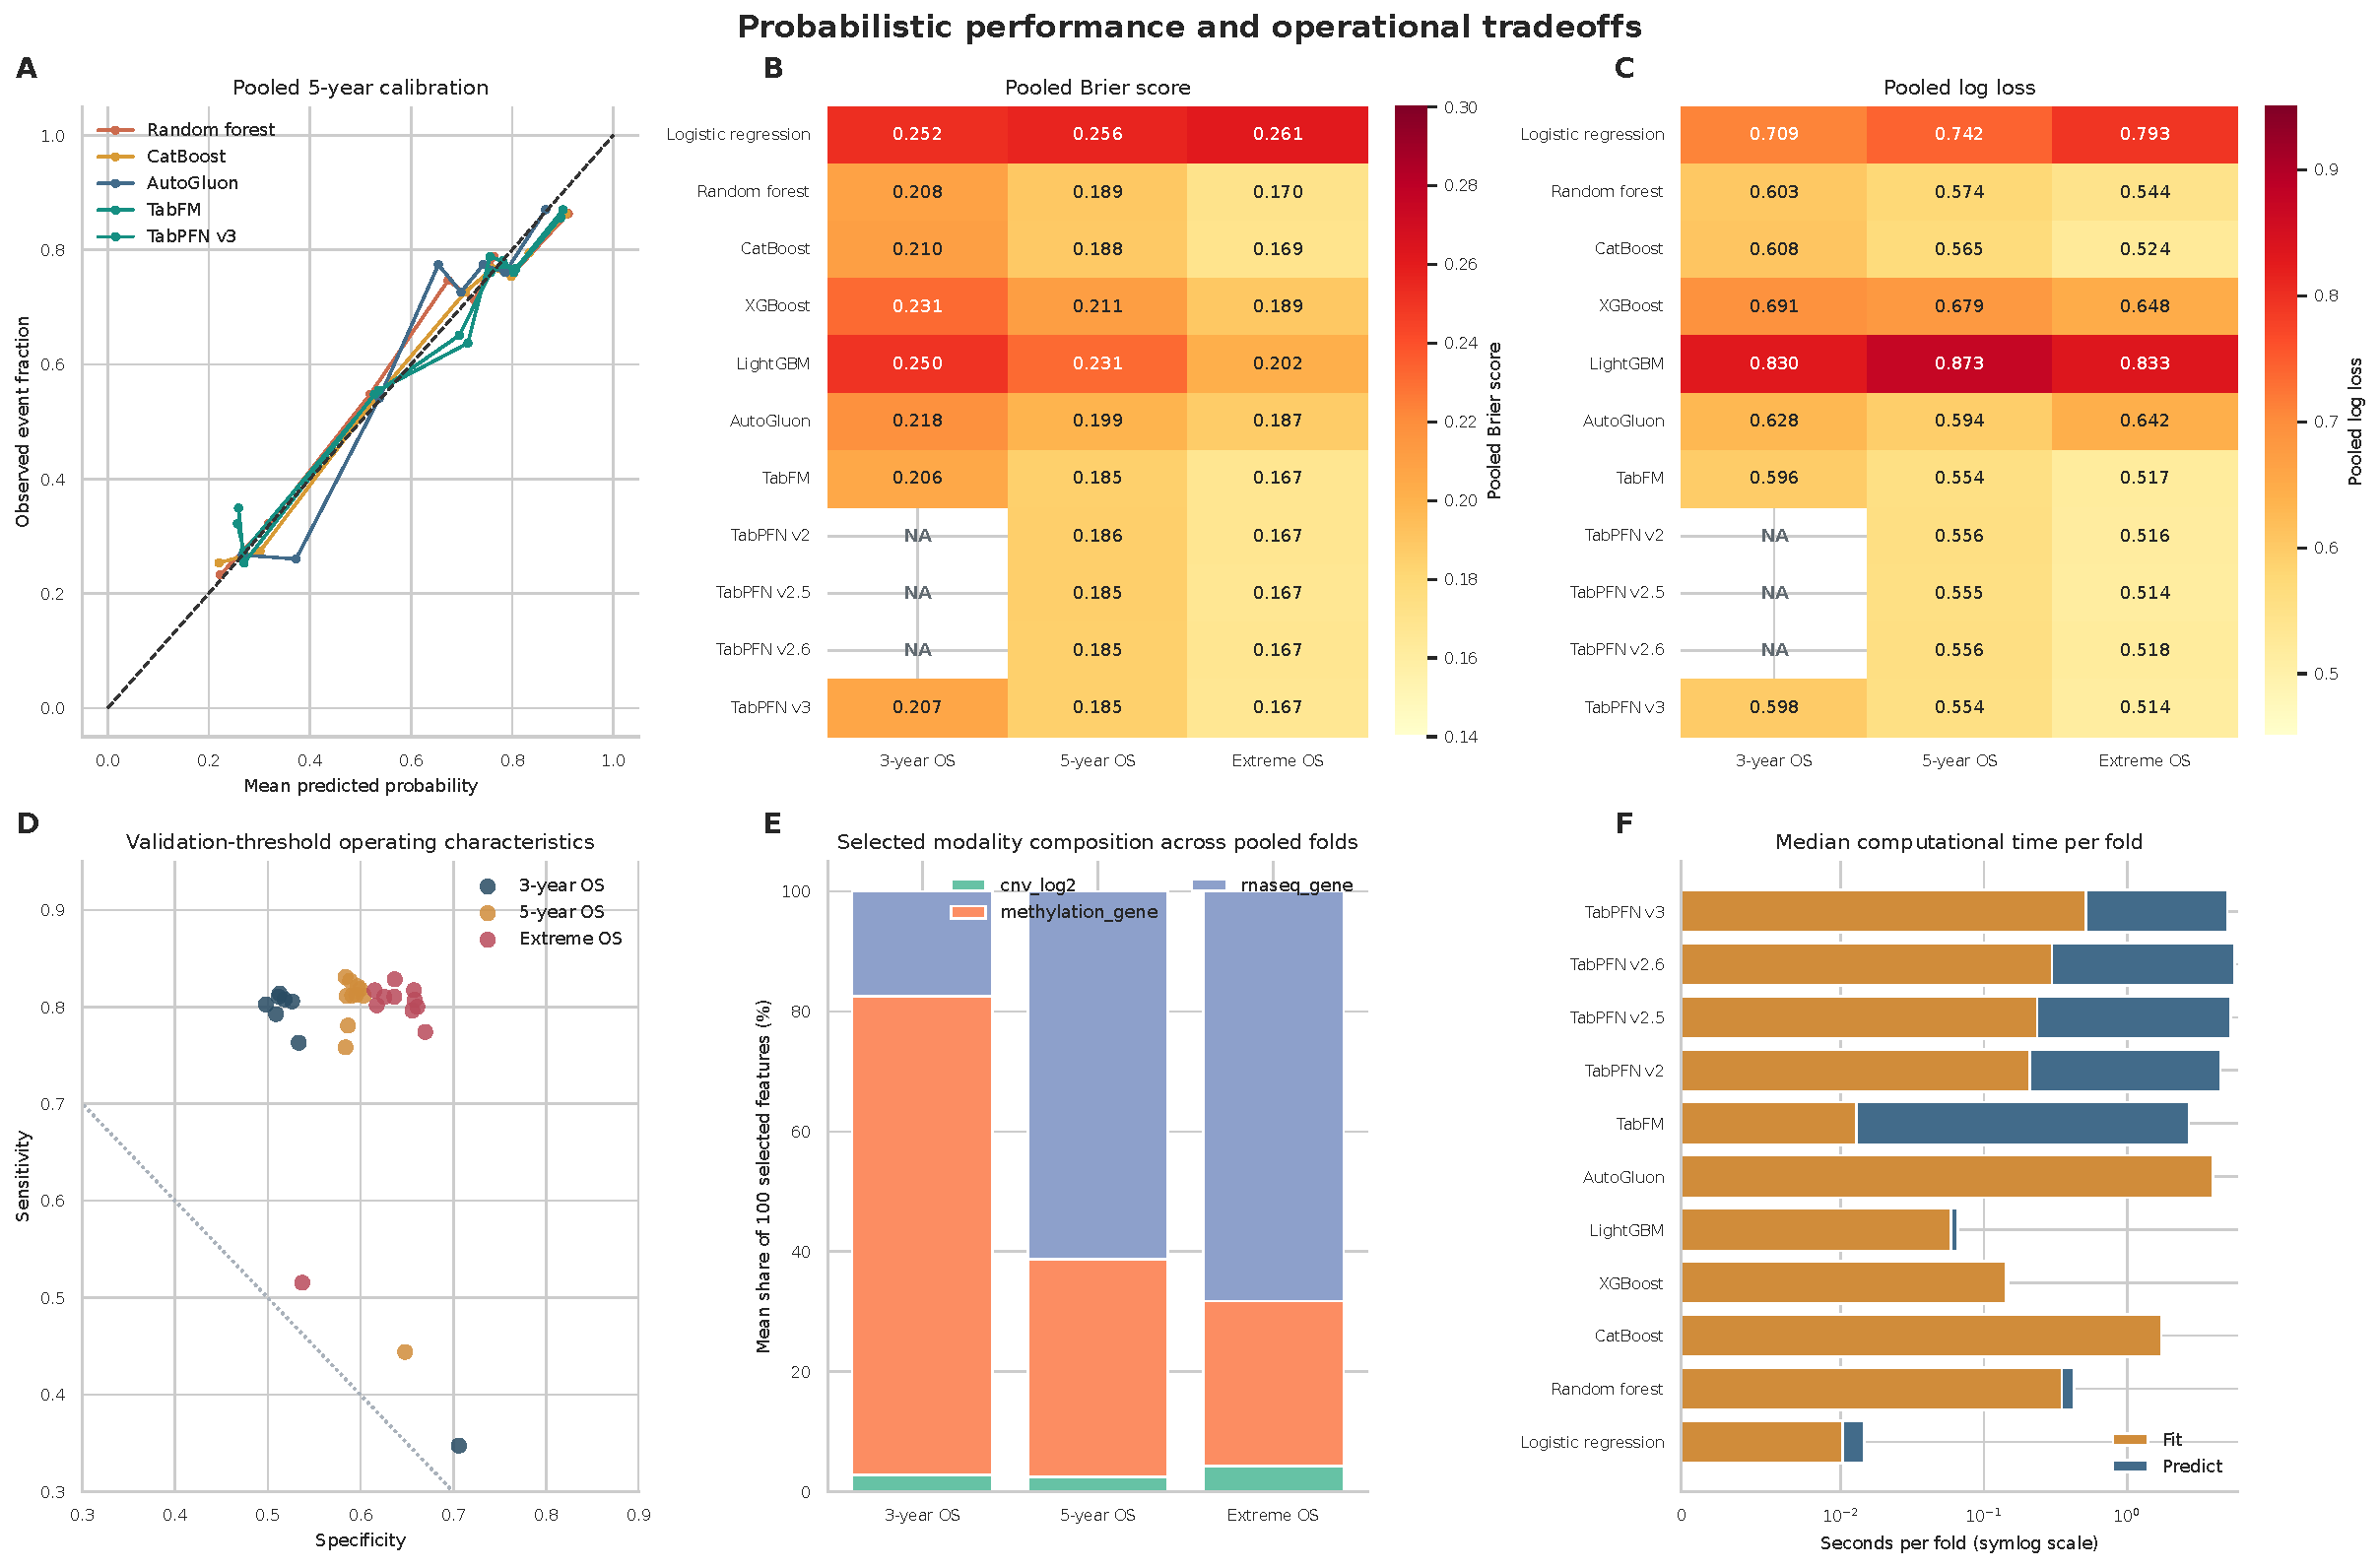
\includegraphics[width=\linewidth,height=0.64\textheight,keepaspectratio]{figures/manuscript/figure_05_probabilistic_and_compute.pdf}
\caption{\textbf{Probability quality and compute.} Calibration curves for pooled 5-year predictions, pooled Brier score and log loss, sensitivity and specificity at validation-selected thresholds, selected-feature modality composition, and median fit and prediction time per fold. Classical models ran locally and foundation models on a separate CPU machine, so runtimes are indicative.}
\label{fig:ed_prob}
\end{figure}


\endgroup
